\documentclass[12pt,letterpaper]{exam}
\usepackage[lmargin=1in,rmargin=1in,tmargin=1in,bmargin=1in]{geometry}
\usepackage{../style/exams}

% -------------------
% Course & Exam Information
% -------------------
\newcommand{\course}{MATH 141: Exam 2}
\newcommand{\term}{Spring --- 2025}
\newcommand{\examdate}{03/07/2025}
\newcommand{\timelimit}{50 Minutes}

\setbool{hideans}{true} % Student: True; Instructor: False


% -------------------
% Content
% -------------------
\begin{document}

\examtitle
\instructions{Write your name on the appropriate line on the exam cover sheet. This exam contains \numpages\ pages (including this cover page) and \numquestions\ questions. Check that you have every page of the exam. Answer the questions in the spaces provided on the question sheets. Be sure to answer every part of each question and show all your work. If you run out of room for an answer, continue on the back of the page --- being sure to indicate the problem number.} 
\scores
\bottomline
\newpage


% -------------------
% Questions
% -------------------
\begin{questions}

% Question 1
\newpage
\question[20] Let $f(x)$ be a twice continuously differentiable function whose \textit{derivative}, $f'(x)$, is plotted below.
	\[
	\fbox{
	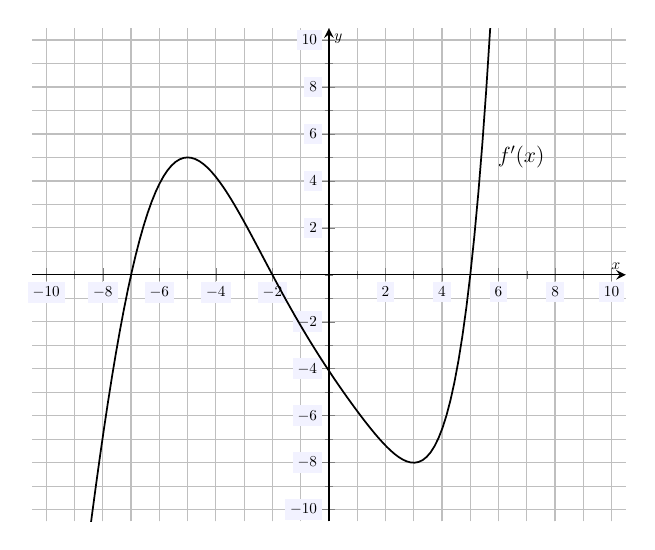
\begin{tikzpicture}[scale=1.1,every node/.style={scale=0.5}]
	\begin{axis}[
	grid=both,
	axis lines=middle,
	ticklabel style={fill=blue!5!white},
	xmin= -10.5, xmax=10.5,
	ymin= -10.5, ymax=10.5,
	xtick={-10,-8,-6,-4,-2,0,2,4,6,8,10},
	ytick={-10,-8,-6,-4,-2,0,2,4,6,8,10},
	minor tick = {-10,-9,...,10},
	xlabel=\(x\),ylabel=\(y\),
	]
	\addplot[line width= 0.02cm,samples=150,domain= -10.5:10.5] ({x},{-4.08789 - 1.80944*x + 0.102687*x^2 - 0.0121406*x^3 + 0.00202778*x^4 + 0.00258073*x^5 + 0.000176215*x^6});
	\node at (6.8,5) {\Large$f'(x)$};
	\end{axis}
	\end{tikzpicture}
	}
	\] 
Based on the plot above, answer the following questions: 
	\begin{enumerate}[(a)]
	\item On what interval(s)---if any---is $f(x)$ increasing? \vfill
	
	\item On what interval(s)---if any---is $f(x)$ decreasing? \vfill
	
	\item On what interval(s)---if any---is $f(x)$ concave up? \vfill
	
	\item On what interval(s)---if any---is $f(x)$ concave down? \vfill
	
	\item Find any critical values for $f(x)$---if any. \vfill
		
	\item Classify any critical values you found in (e). If there were none, state so. \vfill
	
	\item Find the $x$-value(s) for any point(s) of inflection for $f(x)$. \vfill

	\end{enumerate}



% Question 2
\newpage
\question[16] Showing all your work, compute the following limits: \par\vspace{0.3cm}
	\begin{enumerate}[(a)]
	\item $\ds\lim_{x \to \infty} \left[ \ln(9x - 7) - \ln(3x + 5) \right]=$ \vfill
	\item $\ds\lim_{x \to \infty} \dfrac{3 \ln(4x - 2)}{5 \ln(6x + 1)}=$ \vfill
	
	
	\newpage
	
	\phantom{} \par
	\item $\ds\lim_{x \to 0} \dfrac{x + \sin x}{\tan(5x)}=$ \par\vspace{6cm}
	\item $\ds\lim_{x \to 0} (\cos x)^{2/x^2}$ \vfill
	\end{enumerate}



% Question 3
\newpage
\question[16] Find the area of the largest rectangle that has its `upper' vertices on the line $y= 19$ and its `lower' vertices on the function $f(x)= 2x^2 + 1$. 



% Question 4
\newpage
\question[16] An elliptic curve is a special type of curve widely used in cryptography. For its cryptographic applications, one needs to `add' a point on the curve to itself. This process begins with finding the tangent line to the curve at the chosen point. The equation below is an elliptic curve. Find the tangent line to this curve at the point $(-1, 4)$.
	\[
	y^2 + xy + y= x^3 - x^2 - 9x + 9
	\]



% Question 5
\newpage
\question[16] An extension ladder which is 20~feet long is leaning against the wall of a building. Suddenly, the latch of the ladder to the wall detaches and the ladder begins sliding down the wall at 3~ft per second. Simultaneously, the ladder begins to collapse shut at a rate of 2~ft per second. What is the rate at which the bottom of the ladder is moving away from the wall if the ladder is currently extended to a length of 15~ft and is leaning against a point 9~ft up the wall?



% Question 6
\newpage
\question[16] Showing all your work, complete the following parts:
	\begin{enumerate}[(a)]
	\item Find the linearization of $f(x)= \sqrt[4]{x}$ at $x= 16$. \vspace{4cm}\vfill
	\item Use your answer in (a) to approximate $\sqrt[4]{40}$. Express your answer as a decimal. \vfill
	\end{enumerate}

\end{questions}
\end{document}